\documentclass[border=5pt]{standalone}
\usepackage{tikz}
\usepackage{xcolor}

\definecolor{Garnet}{HTML}{73000A}

\tikzset{every node/.append style={rounded corners=0pt}}

\begin{document}
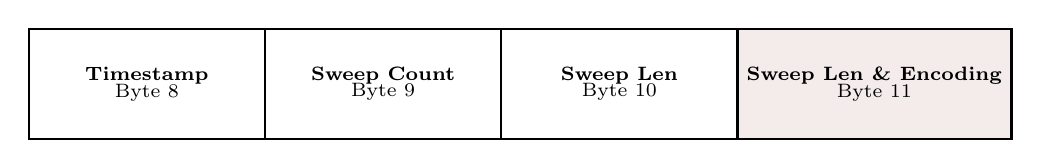
\begin{tikzpicture}[
    block/.style={draw, thick, minimum height=1.4cm, anchor=west, align=center, fill=white, font=\scriptsize},
]

\node[block, minimum width=3.0cm] at (0, 0) {\textbf{Timestamp}\\[-2pt]Byte 8};
\node[block, minimum width=3.0cm] at (3.0, 0) {\textbf{Sweep Count}\\[-2pt]Byte 9};
\node[block, minimum width=3.0cm] at (6.0, 0) {\textbf{Sweep Len}\\[-2pt]Byte 10};
\node[block, minimum width=3.0cm, fill=Garnet!8] at (9.0, 0) {\textbf{Sweep Len \& Encoding}\\[-2pt]Byte 11};

\end{tikzpicture}
\end{document}
